\chapter{Sensitivity Conjecture}

\section{Classic Combinatorial Measures}
Consider a family of functions with signature
\begin{equation}
	f: \{ 0, 1\} \equiv \{ 1, -1\} ^n \rightarrow \{ 0, 1\} 
\end{equation}
the question is then how can we measure the complexity of $f$. 

\subsection{Decision-Tree Complexity}
\begin{definition}
	[Decision Tree Complexity]
	$DT(f)$ is the min-depth of a decision tree that computes $f$.
\end{definition}

As two easy examples, 
\begin{equation}
	DT(\lor) = n \quad \quad \text{and} \quad \quad DT(\land) = n
\end{equation}
for $f = \cdot (x_1, x_2, \dots, x_n)$. Examples here are such that they can be of linear depth or logarithmic. Regardless, these trees depend on all input bits for computation. 


\subsection{Certificate Complexity}
\begin{definition}
	[Certificate Complexity]
	For a specific input
	\begin{equation}
		CC(f, x) = \min\{ |S|: S \text{ is a certificate of $x$} \}
	\end{equation}
	where we say $S\subseteq [n]$ is a certificate for $f$ at $x$ if all inputs that agree with $x$ on $S$ have same $f$ value. Then, for functions, we take
	\begin{equation}
		CC(f) = \max_x CC(f, x)
	\end{equation}
\end{definition}

\paragraph{Example}
Consider $f = \land$. Then $CC(\land, x) = 1$ except for when $x = (1, \dots, 1)$ where 
\begin{equation}
	CC(\land, (1, \dots, 1)) = n
\end{equation}
Thus, 
\begin{equation}
	CC(\land) = n
\end{equation}

\begin{proposition}
	\begin{equation}
		CC(f) \leq DT(f)
	\end{equation}
\end{proposition}

\paragraph{Example} For the majority operation, $MAT_3: \{ 0, 1\} ^3 \rightarrow \{ 0 , 1 \}$. Then, $DT(MAT_3) = 3$ and $CC(MAT_3) = 2$. 

\begin{proposition} 
	\begin{equation}
		DT(f) \leq CC(f) ^ 2
	\end{equation}	
\end{proposition}

\begin{definition}
	[Sensitivity] 
	$S(f, x)$ = \# of neighbors $y$ of $x$ with $f(y) \neq f(x)$. Where `neighbors' mean that $y$ and $x$ differs in exactly one bit. Then, as expected
	\begin{equation}
		S(f) = \max_x S(f, x)
	\end{equation}
\end{definition}

\begin{definition}
	[Hyper Cube]
	A hyper cube $H_n$ has (bit strings) vertices $\{ 0, 1 \} ^ n$. Two vertices are adjacent if they differ in exactly one coordinate. A hypercube is a regular graph with degree $n$. 
\end{definition}

\begin{definition}
	[Sensitivity with Hyper Cube] 
	With help of hyper cube, sensitivity = max over all vertices $x$, \# neighbors of opposite color. 
\end{definition}

\begin{proposition} 
	[Function as Polynomial]
	\label{prop: function as polynomial}
	For any function $f(x_1, \dots, x_n): \{ 0, 1\}^n \rightarrow \{0 , 1\}$, there exists a equivalent representation
	\begin{equation}
		f(x_1, \dots, x_n) \sum_{I \subseteq [n]} C_I \prod_{i \in I} x_i
	\end{equation}
\end{proposition}

\begin{definition}
	[Degree] 
	\begin{equation}
		degree(f): f: \{ 0, 1 \} ^ n \rightarrow \{ 0, 1\} 
	\end{equation}
	is equal to the degree of the polynomial representing $f$, i.e. 
	\begin{equation}
		\max\left\{ |I| : C_I \neq 0 \right\} 
	\end{equation}
\end{definition}

\paragraph{Examples}
\begin{itemize}
	\item $\land_n$, $degree(\land_n) = n$ since $\land_n = x_1 \cdot x_2 \dots x_n$
	\item $\lor_n$, $degree(\lor_n) = n$ since 
		\begin{align}
			\lor_n 
			&= \neg( \land ( \neg x_1, \dots, \neg x_n )) \\
			&= 1 - (1 - x_1) (1 - x_2 ) \dots (1 - x_n)
		\end{align}
\end{itemize}

\begin{proposition}
	Degree and decision tree depth for a function $f: \{0 ,1 \}^ n \rightarrow \{ 0 , 1\}$ satisfies
	\begin{equation}
		degree(f) \leq DT(f)
	\end{equation}	
\end{proposition}
\begin{proof}
	We can write the function as a decision tree, then
	\begin{equation}
		f(x) = \sum_{\ell \in L} (\text{if $x$ leads to } \ell) \cdot (\ell\text{.output})
	\end{equation}
	where $L$ is the set of all leaves in the decision tree. Then, 
	\begin{align}
		f(x) 
		&= \sum_{\ell \in L} (x_{i1} == a_1) (x_{i2} == a_2) \dots (x_{id} == a_d) \cdot (\ell \text{.output} ) \\
		&= \sum_{\ell \in L} \left(a_1 x_{i1} + (1 - a_1) (1 - x_{i1})\right) \dots \left(d x_{id} + ( 1 - a_d) (1 - x_{id})\right)\\
	    \implies & degree(f) \leq DT(f)
	\end{align}
\end{proof}

\begin{proposition} 
	[Summary]
	\begin{equation}
		\left.
		\begin{aligned}
			 S(f) \leq CC(f) \\
			 degree(f)
		\end{aligned} \right\}
		\leq DT(f) \leq CC(f)^2
	\end{equation}
	Note that here we don't know how $degree(f)$ relates to things on the left. This is called sensitivity conjecture. 	
\end{proposition}

\begin{theorem} 
	$degree(f), DT(f), CC(f), RDT(f), QDT(f)$ are all within polynomial factors of each other. 
	\begin{equation}
		\begin{aligned}
			DT(f) \leq CC(f)^2 \\
			degree(f) \leq CC(f) ^ {C_1} \\
			DT(f) \leq degree(f) ^ {C_2}
		\end{aligned}
	\end{equation}
\end{theorem}


\section{Sensitivity Conjecture}
\begin{proposition} 
	[Sensitivity Conjecture (Nisan-Szegedy, 1989)]
	\begin{equation}
		S(f) \geq degree(f)^{C_1}, \quad C_1 \in \real
	\end{equation} 	
	or equivalently, 
	\begin{equation}
		S(f) \geq DT(f) ^{C_2}, \quad C_2 \in \real
	\end{equation}
\end{proposition}

\begin{theorem}
	[Hao Huang, 2019]
	\begin{equation}
		degree(f) \leq S(f) ^ 2
	\end{equation}
\end{theorem}

\begin{theorem}
	[Graph Conjecture Equivalence (Gotsman-Linial, 1992)]
	\paragraph{Statement}
	If for every subgraph of $H$ of $H_n$ of $2^{n - 1} + 1$ vertices, 
	\begin{equation}
		\Delta(H) \geq  g(n) \quad \implies \quad \forall f, S(f) \geq g(degree(f))
	\end{equation}
	where $\Delta (H)$ for a graph $H$ is equal to the max degree of any vertex in $H$. \footnote{We will use this meaning of $\Delta$ through out this chapter.}
	\paragraph{Equivalence}
	Sensitivity Conjecture (1989) is equivalent to ``Graph Conjecture'' proposed by Gotsman-Linial (1992). Huang proved this graph conjecture in 2019. 
\end{theorem}

\begin{proof}
	[TODO]
	will be added later
\end{proof}

\begin{theorem} 
	[Hao Huang, 2019]
	For any subgraph $H$ of $H_n$ of $\geq 2^{n - 1} + 1$ vertices has
	\begin{equation}
		\Delta (H) \geq \sqrt{n}
	\end{equation}	
\end{theorem}
The extra ``$+1$'' part in the formulation plays a significant role. As an example, consider $H$ = the subgraph with vertices 
\begin{equation}
	\{ x \,| \, parity (x) = 0 \} 
\end{equation}
If $|H| = 2^{n - 1}$, i.e. exactly half of the graph, then in this case we can construct $\Delta (H) = 0$. See Figure \ref{fig:n3 parity sub graph} for an example. 

\begin{figure}
	\centering
	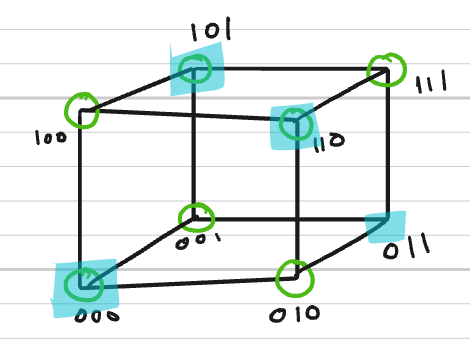
\includegraphics[width=0.4\textwidth]{figs/n3-partity-graph.png}
	\caption{N3 Parity Sub-graph. \label{fig:n3 parity sub graph}}
\end{figure}

\begin{proposition}
	[Observation 1]
	Take any graph $G$, let $A_G$ be its adjacency matrix. Then, \footnote{Here $\lambda_1(G) = $ largest eigenvalue in magnitude. }
	\begin{equation}
		\Delta (G) \geq |\lambda_1 (A_G) | 
	\end{equation}
	Recall that if $A_G$ was regular, we showed that largest eigenvalue = degree of the graph. 
\end{proposition}
\begin{proof}
	Suppose $A_G \bv = \lambda_i \bv$. Let $v_{i^*}$ be the largest entry of $\bv$ in absolute value. 
	\begin{align}
		|\lambda_i| | v_{i^* } |
		&= \left| \sum_{j = 1}^n A_{i^*j} \cdot v_j \right| \\
		&\leq \sum_{j = 1}^n |A_{i^*j}| \cdot |v_j| \\
		&\leq \sum_{j : A_{i^*j} \neq 0} |v_j|  \\
		&\leq \sum_{j: A_{i^* j} \neq 0} |v_{i^*}| \\
		&= degree( i^* ) \cdot | v_{i^*} | 
	\end{align}
	i.e., $|\lambda_1| \leq degree(i^*)$ as wanted. \qed
\end{proof}

\begin{definition}
	[Signed-Adjacency Matrix]
	A matrix ``$B$'' is called a \textit{\textbf{signing}} of a graph $G$ if 
	\begin{equation}
		B_{ij} = (i, j) \text{ edge } ? \in \{0 , 1\} \, : \, 0
	\end{equation}
\end{definition}

\begin{proposition} 
	[Observation 2]
	Take any graph $G$, let $B$ be a signed adjacency matrix of $G$. Then, 
	\begin{equation}
		\Delta (G) \geq |\lambda_1 (B) |
	\end{equation}	
\end{proposition}

\begin{theorem}
	[Cauchy-Interlacing Theorem]
	For a symmetric matrix $M \in \real^{n \times n}$, with eigenvalues
	\begin{equation}
		\lambda_1(M) \geq \lambda_2(M) \geq \lambda_3(M) \geq \dots \geq \lambda_N(M)
	\end{equation}
	its sub-matrix $M_{-1}$ is a $(n - 1) \times (n - 1)$ matrix, obtained by deleting $i$-th row and $i$-th column, with interlacing eigenvalues
	\begin{equation}
		\lambda_i(M) \geq \lambda_i (M_{-1}) \geq \lambda_{i + 1} (M)
	\end{equation}
\end{theorem}

\begin{corollary}
	[General Form, Repeating Interlacing]
	Let $A$ be a symmetric matrix in $\real^{n \times n}$, and $B \in \real^{M \times M}$ be a principal sub-matrix, with
	\begin{equation}
		\lambda_N(A) \leq \lambda_{N - 1} (A) \leq \dots \leq \lambda_1(A)
	\end{equation}
	and 
	\begin{equation}
		\lambda_M(B) \leq \lambda_{M - 1} (B) \leq \dots \leq \lambda_1(B)
	\end{equation}
	Then, 
	\begin{equation}
		\lambda_{N - M + i}(A) \leq \lambda_i(B) \leq_i(A)
	\end{equation}
\end{corollary}

\begin{theorem}
	[Hao Huang, 2019]
	For any subgraph $H$ of $H_n$ of $\geq 2^{n - 1} + 1$ vertices, it has 
	\begin{equation}
		max-degree(H) \geq \sqrt{ n }
	\end{equation}	
\end{theorem}

\begin{proof}
	We know that $max-degree(H) \geq $ largest eigenvalue of $B$ where $B$ is the principal matrix corresponding to vertices in the subgraph of $B_n$. Then, by Cauchy Interlacing Theorem, we have
	\begin{equation}
		\lambda_1(B) \geq \lambda_{N - M + 1}(B_n) \geq \lambda_{2^{n - 1}} (B_n) \geq \sqrt{ n }
	\end{equation}
	This completes the proof. \qed
\end{proof}

\begin{proposition}
	$\forall n, \exists $ a signing $B_n$ of $H_n$ such that 
	\begin{equation}
		B_n^2 = n \cdot \mathbb I _{2^n}
	\end{equation}
\end{proposition}

\begin{proposition}
	If $B_n$ is as above, then it has $2^{n - 1}$ eigenvalues that are $\sqrt {n}$ and the other $2^{n - 1}$ eigenvalues take value $-\sqrt{n}$. 
\end{proposition}

\begin{proof}
	We know that $B_n^2 = n \cdot \mathbb I _ {2 ^ n}$, so every eigenvalue of $B_n$ satisfies $\lambda^2 = n$. This implies 
	\begin{equation}
		\lambda \in \{ \sqrt{n}, - \sqrt{n} \}
	\end{equation}
	Recall that the trace of a symmetric matrix is the sum its eigenvalues. Then here, 
	\begin{equation}
		Tr(B_n) = 0
	\end{equation}
	since $B_n$ must have zero diagonal entries. Hence it must be the case that out of $2^n$ total eigenvalues, half of them are $-\sqrt{n}$ while the other half have value $\sqrt{n}$. \qed
\end{proof}

